\newpage
\section{ Árboles de Decisión y Bosques Aleatorios}
\noindent Sea un vector aleatorio $\textbf{x}$ de longitud $p$ con las variables predictoras e $Y$ la variable respuesta. Se toman $N$ observaciones obteniéndose parejas $(\textbf{x}_i,y_i)$. De esta manera, tenemos que se puede interpretar que $\mathbf{x}_i\in\mathbb{R}^p$.

\noindent Los árboles de decisión son métodos divisivos que dividen el espacio de observaciones $\mathbb{R}^p$ en varias regiones. En cada región, se ajusta un modelo más simple, como una constante.

\noindent La ventaja de este tipo de métodos es que son fácilmente interpretables, ya que pueden ser representados mediante un diagrama de tipo árbol. De esta manera, pueden ser utilizados según \textit{Brown et.al}.\cite{Brown 2004} y \emph{Song Y.Y y Ying, L} \cite{Song 2015} describen los principales objetivos de los árboles de decisión, entre los que se encuentran la selección y evaluación de la importancia de las variables, además de que puede tener fines predictivos o incluso de manejo de los datos, valores perdidos etc... \emph{Nerini, D. y }\cite{Nerini 2007} utilizan árboles de regresión para estimar distribuciones aleatorias e incluso plantean usar técnicas de bagging para mejorar la precisión del modelo. 

\noindent Otra ventaja de este tipo de métodos es que permite trabajar con conjuntos de datos en los que se estudian más variables en comparación de las observaciones, es decir, $p > N$. Por ejemplo, el ejemplo que desarrollan \textit{Díaz-Uriarte y De Andrés} \cite{Diaz 2006}, trabajan con un microarray genético. 

\noindent El problema que más se da en los árboles de decisión es su tendencia al sobre ajuste, ya que de la forma que están conceptualizados, provoca que el sesgo sea pequeño, pero con una gran varianza. Esto se considera en los algoritmos desarrollados durante la sección, normalmente se eliminan particiones que no aporten demasiado. A este proceso se le llama ``poda". 

\noindent Es por esta problemática que se desarrolla el análisis de modelos mediante la descomposición en sesgo y varianza de los mismos. 

\noindent Al haber una cantidad de notación y conceptos notable, se detallan los principales a continuación. 

\subsection*{Conceptos básicos}

\begin{defi}
Se llama \emph{separación, partición o división} de índice $(j,s)$ \cite{Hastie 2001} a la separación que particiona el espacio inicial dado en las siguientes regiones $R_1,R_2$:
\begin{equation}
R_1=\lbrace \mathbf{x}_i \in \mathbb{R}^p/ x_{ij}>s\rbrace \quad R_2=\lbrace \mathbf{x}_i \in \mathbb{R}^p/ x_{ij}\leq s\rbrace
\end{equation}

\noindent Hay que tener en cuenta que esto sería el caso en el que la variable a separar $X_j$ sea continua.

\noindent En el caso de que la variable a particionar sea discreta y no ordinal \emph{Breiman, L.}\cite{Breiman 1984} propone la siguiente solución. Supongamos que $X_j$ toma $L$ valores distintos en un nodo en específico, podemos tomar un conjunto de valores $L_1\subset L$ de tal manera que las regiones que se obtienen son:
\begin{equation}
R_1=\lbrace \mathbf{x}_i \in \mathbb{R}^p/ x_{ij}=l/ l\in L_1\rbrace \quad R_2=\lbrace \mathbf{x}_i \in \mathbb{R}^p/ x_{ij}=l/ l\notin L_1\rbrace
\end{equation}
\end{defi}
\begin{defi}
Se define un \emph{nodo} en un árbol de decisión como cada una de las regiones resultantes después de aplicar una separación.
\end{defi}
\begin{defi}
Se define un \emph{nodo terminal o nodo hoja}    \cite{Brown 2004} en un árbol de decisión como cada una de las regiones finales resultante de la partición del espacio de observaciones.
\end{defi}
\begin{defi}
Llamaremos tamaño del árbol $T$, $|T|$ al número de nodos terminales. \cite{Hastie 2001}
\end{defi}
\begin{defi}
Se llama profundidad del árbol al número máximo que de divisiones necesarias para llegar a un nodo terminal \cite{Hastie 2001}. \emph{En el caso del diagrama que se incluye después se dan 3 divisiones del espacio tanto para llegar a $R_4, R_5$}
\end{defi}
\noindent Las  siguientes imágenes procedentes de \textit{Hastie et. al.}\cite{Hastie 2001} muestran el diagrama resultante tras dividir el espacio de observaciones mediante un árbol. 

\begin{figure}[h]
 \centering
  \subfloat[División de $\mathbb{R}^p$]{
   \label{f:división}
    \includegraphics[width=0.4\textwidth]{Documentos Extra/Imagenes/Regiones árboles.png}}
  \subfloat[Diagrama resultante]{
   \label{f:diagrama arbol}
    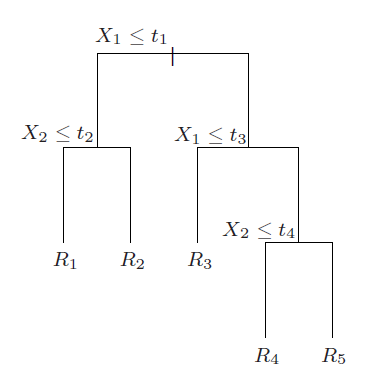
\includegraphics[width=0.4\textwidth]{Documentos Extra/Imagenes/Diagrama de arbol.png}}
 \caption{Representación de la división de $\mathbb{R}^p$ y el diagrama de árbol resultante}
 \label{f:MARC1}
\end{figure}

\noindent Como se puede ver, cada uno de los nodos terminales representan cada una de las regiones en las que se ha separado el espacio de observaciones. 

\noindent Dependiendo del tipo de variable respuesta, se utiliza un \emph{Árbol de regresión} cuando se busca predecir una variable continua, y un \emph{Árbol de clasificación} cuando se busca clasificar variables discretas. En nuestro caso, los algoritmos que se describirán pueden manejar tanto variables de entrada discretas como continuas. Se detallará el caso en el que las variables de entrada son continuas.

\noindent \emph{Observación:} La razón de usar particiones binarias es que son fáciles de entender y manejar. Esto hace que los árboles de decisión sean más fáciles de usar y nos ayuda a comprender las áreas o regiones que hemos creado al particionar. 

\subsection*{Sesgo y varianza de un modelo}

\noindent Un aspecto en el que no se ha indagado en el trabajo por ahora es en la capacidad predictiva de los modelos. Es decir, la capacidad de obtener, dadas nuevas observaciones $\mathbf{x}_0$ de las variables predictoras, el valor que tendría la variable respuesta $Y$. La razón de que se detalle ahora es que los árboles son modelos los cuales tienden al sobreajuste y algunos autores como \emph{Breiman, L.}\cite{Breiman 1984} o \emph{Divakaran, S.}\cite{Divakaran 2022} proponen mecanismos para evitar dicha situación e incluso proponen utilizar técnicas alternativas basadas en los árboles de decisión como los  \emph{Bosques aleatorios}\cite{Breiman 2001}. 

\noindent Supóngase variable respuesta sigue un modelo del tipo $Y=f(\mathbf{x})+\varepsilon$, en el que la variable aleatoria $\varepsilon\sim N(0,\sigma^2)$ y la variable respuesta $Y\sim N(f(\mathbf{x}),\sigma^2)$ conociendo el vector de variables predictoras. Por ejemplo, la $f(\mathbf{x})$ es una función lineal y la variable respuesta $Y$ es continua, se estaría ante un modelo de regresión lineal. 

\noindent Consideremos que se toma una muestra con  $N$ observaciones, obteniéndose una matriz de datos $\mathbf{X}$, la matriz de respuesta $\mathbf{Y}$ y que se ajusta el modelo y sus parámetros conocidas conociendo estas $N$ observaciones. Entonces, para una nueva observación de las variables predictoras $\mathbf{x}_0$, se puede definir el siguiente concepto \cite{Hastie 2001, Lawless 2010}.

\begin{defi}
Se llama \emph{error de predicción esperado} de la observación $\mathbf{x}_0$ a la siguiente expresión:
\begin{equation}
EPE(\mathbf{x}_0)=\mathbb{E}((Y-\hat{Y})^2|\mathbf{x}=\mathbf{x}_0)=\mathbb{E}((Y-\hat{f}(\mathbf{x}_0))^2)
\end{equation}
\end{defi}
\noindent De esta manera, se tiene una forma de medir el rendimiento predictivo de un modelo. En aplicaciones de aprendizaje automático, donde el principal el objetivo es la predicción, dividimos los datos en conjuntos de entrenamiento y validación. Después de ajustar el modelo, evaluamos qué tan bien puede predecir utilizando una muestra separada de los datos de entrenamiento. Esto nos ayuda a estimar el error esperado en las predicciones.

\noindent Además, este error de predicción se puede descomponer de manera sencilla 
\begin{propo}
El error de predicción esperado se puede dividir en un termino irreducible, el sesgo del modelo y la varianza \cite{Hastie 2001}:
\begin{equation}
EPE(\mathbf{x}_0)=\sigma_{\varepsilon}^2+Sesgo(\hat{f}(\mathbf{x}_0))^2+Var(\hat{f}(\mathbf{x}_0))
\end{equation}
\noindent Donde el $Sesgo(\hat{f}(\mathbf{x}_0))=\mathbb{E}(f(\mathbf{x}_0)-\hat{f}(\mathbf{x}_0))$.
\begin{proof}
\begin{align*}
\mathbb{E}((Y-\hat{f}(\mathbf{x}_0))^2)&=\mathbb{E}((Y-f(\mathbf{x}_0)+f(\mathbf{x}_0)-\hat{f}(\mathbf{x}_0))^2)=\\
&=\mathbb{E}(\varepsilon^2)-2\mathbb{E}(\varepsilon\cdot(f(\mathbf{x}_0)-\hat{f}(\mathbf{x})_0))+\mathbb{E}((f(\mathbf{x}_0)-\hat{f}(\mathbf{x}_0)^2)\\
&=\sigma^2+\mathbb{E}((f(\mathbf{x}_0)-\hat{f}(\mathbf{x}_0))^2)
\intertext{El segundo término es el error cuadrático medio de un estimador, luego se obtiene que:}
\mathbb{E}((Y&-\hat{f}(\mathbf{x}_0))^2)=\sigma^2+Sesgo(\hat{f}(\mathbf{x}_0))^2+Var(\hat{f}(\mathbf{x}_0))
\end{align*}
\end{proof}
\end{propo}

\noindent Estos dos parámetros están íntimamente relacionados con la complejidad del modelo, ya que cuanto más complejo sea el modelo, el sesgo se reduce de manera importante. Esto es debido a que los puntos del conjunto de entrenamiento están bastante cerca de las funciones aproximadas, en cambio la varianza se dispara, lo que implica que a la hora de hacer predicciones estas no sean lo mejor posible \cite{Neural Designer}. 

\noindent Para el caso en el que tengamos un modelo de regresión lineal que \emph{Hastie et. al.} \cite {Hastie 2001} desarrolla, se ve que la varianza del error esperado medio en observaciones del conjunto de entrenamiento depende de $\frac{p}{N}$, y el sesgo de $\frac{1}{N}$. Por tanto, a mayor numero de observaciones y menor de variables predictoras mejor. Esto se puede observar en el siguiente gráfico que incluyen \emph{Hastie et.al.} \cite{Hastie 2001} de manera que se puede ver a mismo número de observaciones que pasa si aumentamos las variables observadas. La línea roja representa lo que ocurre con el error de predicción en observaciones fuera del conjunto de ajuste y la azul representa dentro del conjunto de ajuste. 

\begin{figure}[h]
\centering
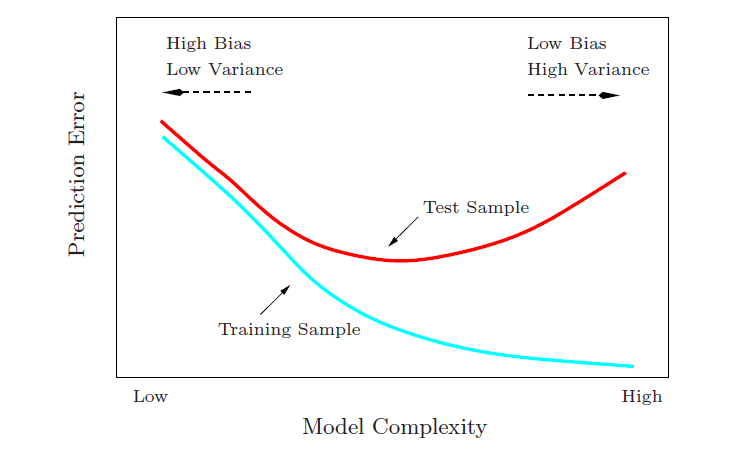
\includegraphics[scale=0.5]{Documentos Extra/Imagenes/Bias-Variance-Tradeoff.png}
\end{figure}
 
\noindent En la figura se puede observar lo qué ocurre en el caso de que un modelo esté en una situación de infraajuste en la parte izquierda, no se ajusta el modelo ni para muestras dentro de los datos ni en el caso que cojamos una que no esté en los datos. En el caso contrario tenemos la parte derecha donde el modelo se ajusta demasiado a los datos recogidos y no tiene capacidad predictiva. Esto puede ocurrir por lo siguiente; que la complejidad del modelo en relación con la cantidad de muestras sea demasiada alta. 

\noindent Como hemos dicho antes el crecimiento de los árboles tanto de regresión como de clasificación busca sobreajustarse. En la siguiente parte veremos como hay distintos algoritmos que buscan evitar dicho sobreajuste. 

 
%\noindent Esta parte se va utilizar, tanto en los árboles como en los random forests, ya que son métodos que buscan con un conjunto relativamente pequeño de observaciones en relación con el numero de variables observadas obtener un modelo que no tenga un sobre ajuste excesivo. De hecho, para hacer crecer un árbol, se busca hacerlo crecer hasta un punto de sobre ajuste y luego se irá ``podando" de la manera que se definirá más tarde para evitar dicho sobre ajuste introduciendo algo de sesgo. 

\subsection{Árboles de regresión }
\noindent A continuación, examinemos el  proceso de crecimiento de un árbol de regresión. En este caso, se considera un vector aleatorio $\mathbf{x}$ con $p$ variables predictoras y una variable respuesta continua $Y$. En particular, se desarrollan los conceptos y proceso llevado a cabo en el algoritmo \emph{CART} de \emph{Breiman, L.} \cite{Breiman 1984}. 

\noindent Supongamos que hemos establecido un número máximo de particiones $M=|T|$. En consecuencia, el objetivo del árbol de decisión es dividir el espacio de observaciones en regiones $R_m$ para $m=1,\ldots, M$. Cada región $R_m$ está asociada a su \emph{función característica}, que denotaremos como $\mathbf{1}_m$.

\noindent En el caso de que se tomen $N$ observaciones, podemos definir el estimador resultante $\hat{f}(\mathbf{x})$ de la siguiente manera:

\begin{equation}
\hat{f}(\mathbf{x})=\sum_{m=1}^M \hat{f}_m(\mathbf{x})\cdot \mathbf{1}_m(\mathbf{x})
\end{equation}

\noindent Esto significa que en cada región $R_m$, se realiza una regresión utilizando los datos correspondientes a esa región. Generalmente, se busca una aproximación lo más sencilla posible en cada $R_m$, por ejemplo, utilizando una constante. \cite{Hastie 2001,Biau 2016}.

\noindent Si se aplica el método de los mínimos cuadrados, con la restricción requerida, se pueden definir las constantes $\hat{c}_m$ de la siguiente manera \emph{(Para ver demostración completa véase la sección de 9.1 \cite{Breiman 1984})} :
\begin{equation}
\hat{c}_m=\dfrac{1}{N_m}\sum_{i/\mathbf{x}_i\in R_m} y_i
\end{equation}

\noindent Donde $N_m$ es el número de observaciones del total que hay en $R_m$. Es decir, $\hat{c}_m$ es la media muestral de las respuestas de las observaciones pertenecen a la región y esto provoca que $\hat{f}(\mathbf{x})=\sum_{m=1}^M \hat{c}_m \cdot \mathbf{1}_m(\mathbf{x})$. Es decir, la predicción $\hat{y}$ para un $\mathbf{x}\in R_m$ otorgada por el modelo es $\hat{c}_m$. \cite{Hastie 2001, Breiman 1984}

\noindent Una vez se conoce como se va a dar la estimación final, hay que saber cómo llegar a la mejor partición. A este proceso de elegir las particiones y elegir dichas particiones $(j,s)$. 

\noindent En regresión, hay que elegir $j$ y $s$ de tal manera que las regiones resultantes $R_{m_1},R_{m_2}$ son aquellas en las que se minimiza la siguiente expresión \cite{Breiman 1984}:
\begin{equation}
\sum_{i/\mathbf{x}_i\in R_{m_1} } (y_i-\hat{c}_{m_1})^2+\sum_{i/\mathbf{x}_i\in R_{m_2} } (y_i-\hat{c}_{m_2})^2
\end{equation}

\noindent Es decir, el objetivo es encontrar las separaciones que minimicen la suma de los errores cuadráticos. A este criterio se le llama \emph{CART}\cite{Breiman 1984}, aunque \emph{Biau, G. y Scornet, E.}\cite{Biau 2016} lo plantea de manera distinta. Podemos definir el error cuadrático medio de cada región de la siguiente manera \cite{Hastie 2001}.

\begin{defi}
Se llama error cuadrático medio de una región $R_m$ a $Q_m(T)=\frac{1}{N_m}\sum_{i/\mathbf{x}_i\in R_m}(y_i-\hat{c}_m)^2$ \cite{Hastie 2001}.
\end{defi}

\noindent Por tanto, podemos definir una función de coste general 
\begin{equation}
Q(T)=\sum_{m=1}^M\frac{1}{N_m}\sum_{i/\mathbf{x}_i\in R_m} (y_i-\hat{c}_m)^2
\end{equation}


\noindent Ya que el error cometido medio en el espacio de observaciones es la media de todos los errores cometidos en cada una de las regiones en las que se particiona el espacio \cite{Breiman 1984}. 


\noindent En el caso de que $\mathbf{x}_0\in R_m$ y las mismas suposiciones que en la sección anterior, una observación que no está entre las recogidas en la matriz de datos, el error de predicción esperado cumple lo siguiente:
\begin{align}
EPE(\mathbf{x}_0)&=\sigma^2+(Sesgo(\hat{f}_m(\mathbf{x}_0)))^2+Var(\hat{f}(\mathbf{x}_0))
\intertext{Como $\mathbf{x}_0\in R_m$ entonces, se tiene que:}
EPE(\mathbf{x}_0)&=\sigma^2+(Sesgo(\hat{f}_m(\mathbf{x}_0)))^2+Var(\hat{f}_m(\mathbf{x}_0))
\intertext{En particular, $\hat{f}_m(\mathbf{x})=\hat{c}_m$, por tanto, es un estimador insesgado cuya varianza es $\frac{\sigma^2}{N_m}$ ya que procede de hacer una media muestral la variable $Y\sim N(0,\sigma^2)$, por tanto:}
EPE(\mathbf{x}_0)&=\sigma^2+\dfrac{\sigma^2}{N_m}
\end{align}

\noindent Por tanto, hacer crecer un árbol, es decir, hacer que tenga más nodos términales, va a provocar que $N_m$ sea menor, por lo tanto, hacer crecer un árbol demasiado hace que estemos en un caso de sobre ajuste. Es por ello, que se crean métodos como la \emph{poda}.

\noindent Para empezar, hay que definir lo que significa la poda de un árbol. 
\begin{defi}
Se llama \emph{poda} al proceso en el que dado un árbol inicial de tamaño $T_0$ se revierten ciertas particiones terminales que no aportan en la relación coste-complejidad, es decir, aumentan demasiado la complejidad (\emph{Aumentando la varianza}), sin reducir el coste en exceso. 
\end{defi}


\noindent \emph{Divakaran, S. }\cite{Divakaran 2022} y \emph{Breiman, L.}\cite{Breiman 1984}, proponen añadir un término al coste del árbol. 
\begin{equation}
Q_{\alpha}(T)=\sum_{m=1}^M\frac{1}{N_m}\sum_{i/\mathbf{x}_i\in R_m} (y_i-\hat{c}_m)^2+\alpha|T |
\end{equation}

\noindent Donde $\alpha$ es un término para controlar la complejidad del árbol, es decir, $\alpha=0$ es el criterio habitual, mientras que cuanto mayor sea, más pequeños serán los árboles, ya que penaliza más el tamaño.  

\noindent El proceso que sugiere \emph{Divakaran S.}\cite{Divakaran 2022}, basado en el que da \emph{Breiman L.}\cite{Breiman 1984} viene dado por los siguientes pasos:
\begin{itemize}
\item Primero prepara el conjunto de datos para poder realizar validación cruzada \emph{(Véase el capítulo 7 de \cite{Hastie 2001}, en particular el método de K-folds)}
\item Se hace una partición binaria hasta tener un árbol de gran tamaño $T_0$,parando con cualquiera de los criterios habituales como pueden ser un máximo de nodos terminales o un mínimo de observaciones por nodo. 

\item Se aplica la poda al árbol utilizando el coste que penaliza el tamaño del propio árbol, teniendo en cuenta el parámetro $\alpha$. 

\item \emph{Divakaran S.}\cite{Divakaran 2022} aplica el método de K-folds para elegir el parámetro $\alpha$
\end{itemize}

\noindent Este método nos devuelve un subárbol $T_{\alpha}$ con el $Q_{\alpha}(T)$ menor posible. En caso de que $\alpha=0$, $T_{\alpha}=T_0$.

\noindent En este caso, se está teniendo un intercambio entre varianza y sesgo, de manera que un árbol tiene menor sesgo, ya que se ajusta de mejor manera a los datos de ajuste pero a la hora de hacer predicciones no son las mejores. De esta manera, se da a cambio de un poco más de sesgo, se reduce la varianza. (\emph{Véase el capitulo 7 de \cite{Hastie 2001} o el capitulo 5 de \cite{James 2013} })

\noindent Otro algoritmo de selección de las particiones es el algoritmo \emph{C4.5} de \emph{Quinlan, J}\cite{Quinlan 2014} y aunque se desarrollará aplicado a árboles de clasificación, su implementación para árboles de regresión es análoga, cambiando únicamente el criterio, ya que el dado no es válido para variables respuesta continuas. 

\subsection{Árboles de Clasificación}

\noindent Sea ahora el caso en el que las variables predictoras son como antes, dadas por un vector aleatorio $\mathbf{x}$ de longitud $p$ , discretas o continuas de manera indiscretas, pero en el que la variable respuesta es una variable aleatoria con $L$ posibles valores.

\noindent Tómense ahora $N$ observaciones simultáneas del vector $\mathbf{x}$ y la variable respuesta $Y$ para el cual se ha hecho crecer un árbol $T$ de tamaño $M$, entonces, podemos denotar de la siguiente manera \cite{Divakaran 2022, Brown 2004}
\begin{equation}
\hat{p}_{lm}=\text{Proporción de observaciones en las que $y_i=l$, en la región $R_m$.}
\end{equation}

\noindent Teniendo en cuenta esto, se pueden definir los siguientes conceptos.
\begin{defi}
Se dice que un nodo correspondiente a la región $R_m$ es puro, si $\exists l_0/ p_{l_0 m}=1$ y $\hat{p}_{lm}=0 \quad \forall l\neq l_0$ \cite{Divakaran 2022, Hastie 2001, James 2013, Brown 2004}. 
\end{defi}

\begin{defi}
Se define la \emph{impureza de un nodo}, correspondiente a la región $R_m$ como \cite{Brown 2004}:
\begin{equation}
1-\max_{l\in L} \hat{p}_{lm}
\end{equation}
\noindent Es decir, si se hablara de coste, estamos asumiendo que en esa región $R_m$, la $l$ tal que $\hat{p}_{lm}$ es máxima es la correcta. Entonces, la impureza se puede interpretar como la ``probabilidad" de error. 
\end{defi}
\noindent Otra forma de medir la impureza son el índice Gini y la entropía. \emph{Hastie et. al.} y \emph{Divakaran, S.} \cite{Hastie 2001, Divakaran 2022}, definen el índice Gini de la siguiente manera:
\begin{defi}
Se llama \emph{índice Gini} de una región $R_m$ a la siguiente expresión \cite{Hastie 2001, James 2013}:
\begin{equation}
G=\sum_{l=1}^L\hat{p}_{lm}(1-\hat{p}_{lm})
\end{equation}
Esta medida es la varianza que tiene un nodo. 
\end{defi}

\noindent Con esta medida se desarrolla el algoritmo de \emph{CHAID}, en el que la variable $X_j$ que se elige, se elige mediante un test de similitud y aquellas particiones de las planteadas que sean demasiado parecidas se fusionan.   \emph{(Véase \cite{Kass 1980} para leer el desarrollo inicialmente propuesto por Kass G.V.)} 

\begin{defi}
Se llama \emph{entropía} a la siguiente medida \cite{Brown 2004}:
\begin{equation}
H(\hat{p}_{lm})=-\hat{p}_{lm}log_2(\hat{p}_{lm})-(1-\hat{p}_{lm})log_2(1-\hat{p}_{lm})
\end{equation}

\noindent Esta medida toma valores en el intervalo $[0,1]$ siendo $H(\frac{1}{2})=1$ el máximo cuando hay tantas clasificaciones posibles correctas como incorrectas. Y tiene el mínimo en el 0 y el 1 donde toma el valor 0 ya que en ambos casos hay sólo clasificaciones erróneas o correctas.

\noindent Entonces, se puede definir la entropía total del nodo $m$ como la siguiente expresión:
\begin{equation}
H(R_m)=-\sum_{l=1}^L(\hat{p}_{lm})log(\hat{p}_{lm})
\end{equation}

\noindent Esta medida nos da una idea de la \emph{impureza} del nodo, es decir de la cantidad de clasificaciones distintas que podrían hacerse en ese nodo. 
\end{defi}

\noindent El algoritmo \emph{C4.5} de \emph{Quinlan J.R.} \cite{Quinlan 2014} hace uso de un criterio para hacer crecer el árbol de clasificación. Pero para ello, hay que definir el concepto de ganancia de información y de ratio de ganancia.
\begin{defi}
Supóngase que se tiene un nodo padre que se divide en $m$ nodos hijos, entonces la \emph{ganancia de información } se define de la siguiente manera: 
\begin{equation}
Ganancia=H(padre)-\sum_{i=1}^M \dfrac{N_m}{N_{padre}}H_i
\end{equation}
\noindent Es decir, es la entropía del nodo padre menos la media ponderada de las entropías de cada uno de los nodos \cite{Brown 2004}. 
\end{defi}

\begin{defi}
Llamamos ratio de ganancia a la siguiente cantidad que está entre 0 y 1 \cite{Brown 2004}:
\begin{equation}
\dfrac{Ganancia}{H_{padre}}
\end{equation}
Por tanto, un valor cercano a 1  aporta un gran cambio y un valor cercano a 0 es que casi la ganancia es nula.   
\end{defi}

\noindent Teniendo esta medida se puede plantear el método de construcción de árboles \emph{C4.5} \cite{Loh 2014} de la siguiente manera.

\noindent Para cada tipo de variable se da un tipo sistemático de particiones del espacio, en el caso de que $X_j, j=1\ldots p$ sea una variable aleatoria discreta sin orden, que toma $l$ valores distintos en el nodo que se va a particionar, entonces se hacen $l$ particiones y en cada partición tomará cada uno de los valores. 

\noindent En el caso de que la variable $X_j$ sea continua se hace una partición binaria a partir de la media en el nodo padre. Es decir, tomamos la regla discriminante $X_j>c$, $X_j\geq c$, donde $c$ es la media de la variable $X_j$ en el nodo padre. 

\noindent Una vez calculada las particiones para cada una de las variables, se calcula la ganancia de cada una de las particiones, y se toma la que mayor ratio de ganancia tenga. 

\noindent De esta manera, se obtiene otro algoritmo voraz para el crecimiento del árbol. Al igual que en el resto, se puede hacer un proceso de poda para evitar el sobre ajuste. 


\subsection{Algoritmo Random Forest}

\noindent El término bosque aleatorio se puede referir a dos conceptos distintos, uno el hecho de utilizar varios árboles sin importar como se obtienen y luego utilizar la media de los resultados o el voto por mayoría dependiendo del tipo de variable respuesta sea discreta o continua. 

\noindent El término \emph{random forest} se refiere al algoritmo de \emph{Breiman, L.} \cite{Breiman 2001}. Este tipo de algoritmo si hace hincapié en el  método con el se construyen los árboles. 

\noindent El proceso de construcción y de utilización de los \emph{random forest} lo detallan \emph{Biau, G. , Scornet, E. y Breiman, L.}\cite{Biau 2016,Breiman 2004} :
\begin{itemize}
\item En cada árbol se utiliza una muestra aleatoria sin reemplazamiento del conjunto de datos iniciales. La razón es buscar una muestra \emph{bootstrap} de los datos iniciales \emph{(Véase \cite{Hesterberg 2011} para más detalles de la técnica.)}
\item Se establece un número $j_{try}$ por el usuario. Para cada partición a realizar se escogen de manera aleatoria $j_{try}$ variables y se elige la que más se ajusta al criterio dado. Y se hace crecer el árbol todo lo necesario o hasta un criterio dado por el usuario. 
 
\item Una vez se tienen crecidos los árboles, se toma como predicción de una nueva observación la media de las predicciones de los datos en el caso de que la variable respuesta sea continua. En el caso de que sea una variable discreta, se toma el voto por mayoría, es decir se toma el valor que más veces haya salido en todos los árboles. 
\end{itemize}

\noindent \emph{Breiman, L.} \cite {Breiman 2004} detalla las propiedades básicas de un random forest. Entre estas propiedades se encuentran el sesgo, la varianza y sus acotaciones. Además \emph{Biau G. y Scornet, E. }\cite{Biau 2016} destacan que no es habitual ver un estudio profundo de estos métodos debido 

\noindent \emph{Breiman, L.} \cite{Breiman 1996} llama a este tipo de métodos los métodos de \emph{bagging}. Este tipo de métodos lo que busca es reducir la varianza de métodos con sobreajuste utilizando la media y el teorema central del límite de manera que el predictor final es media de los predictores, lo que consigue reducir la varianza de manera importante. Además detalla que en los casos en los que los predictores no tengan esa varianza alta en comparación con el sesgo, el método de \emph{bagging} no tiene un gran impacto e incluso puede resultar perjudicial debido al incremento de coste computacional que se puede dar